\documentclass[tikz,border=6pt]{standalone}
\usepackage{tikz}
\usetikzlibrary{positioning, shapes, arrows.meta, calc}
\begin{document}
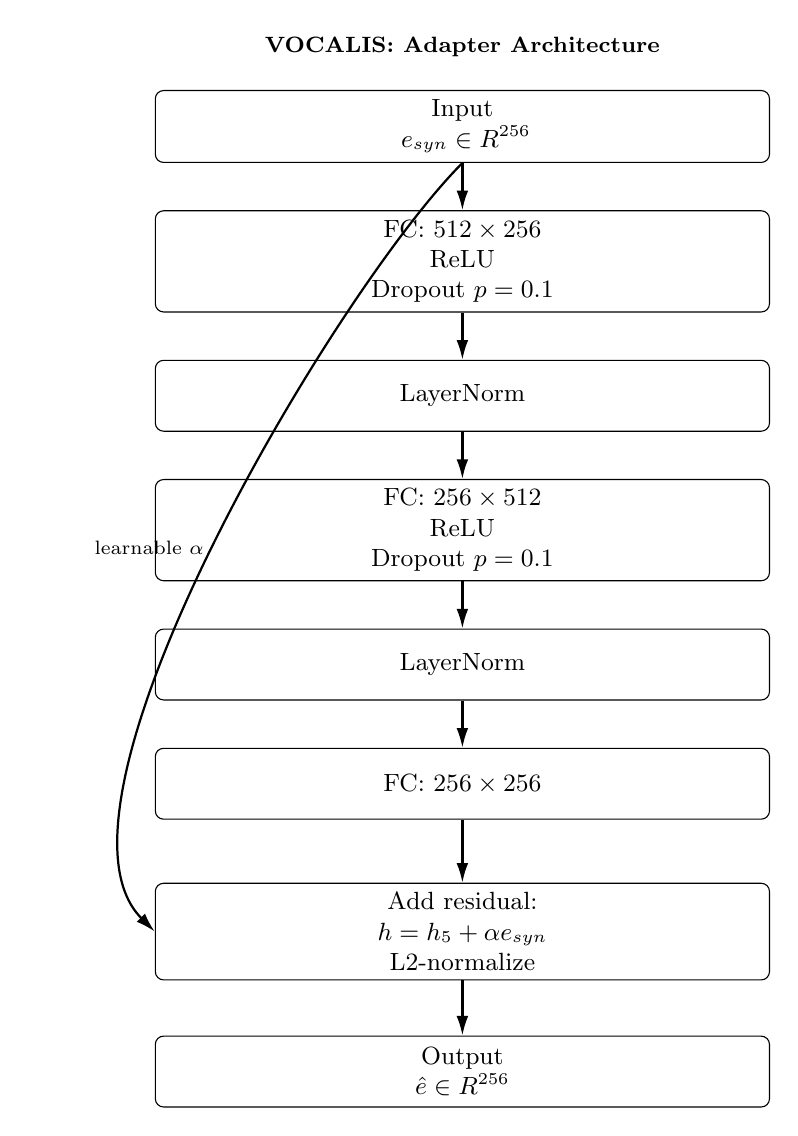
\begin{tikzpicture}[
  block/.style={draw, rectangle, rounded corners=3pt, minimum width=7.8cm, minimum height=0.9cm, align=center, font=\small},
  arrow/.style={-{Latex[length=2.5mm,width=1.5mm]}, line width=0.8pt}
]
% Nodes (vertical)
\node[block] (in) {Input \\ $\;e_{\text{syn}}\in\mathbb{R}^{256}$};
\node[block, below=6mm of in] (fc1) {FC: $512\times256$ \\ ReLU \\ Dropout $p=0.1$};
\node[block, below=6mm of fc1] (ln1) {LayerNorm};
\node[block, below=6mm of ln1] (fc2) {FC: $256\times512$ \\ ReLU \\ Dropout $p=0.1$};
\node[block, below=6mm of fc2] (ln2) {LayerNorm};
\node[block, below=6mm of ln2] (fc3) {FC: $256\times256$};
\node[block, below=8mm of fc3] (add) {Add residual: \\ $h = h_5 + \alpha e_{\text{syn}}$ \\ L2-normalize};
\node[block, below=7mm of add] (out) {Output \\ $\hat{e}\in\mathbb{R}^{256}$};

% Arrows
\draw[arrow] (in) -- (fc1);
\draw[arrow] (fc1) -- (ln1);
\draw[arrow] (ln1) -- (fc2);
\draw[arrow] (fc2) -- (ln2);
\draw[arrow] (ln2) -- (fc3);
\draw[arrow] (fc3) -- (add);
\draw[arrow] (add) -- (out);

% Residual arrow from input to add (curved)
\draw[arrow] (in.south) .. controls +(-1.6cm,-1.6cm) and +(-1.6cm,1.6cm) .. node[left, font=\scriptsize] {learnable $\alpha$} (add.west);

% Title
\node[above=3mm of in, font=\bfseries\footnotesize] {VOCALIS: Adapter Architecture};

\end{tikzpicture}
\end{document}
